\section{Instruction Set and Code Development} \label{sec:code}
\subsection{Instructions}
The Insctructions implemented are freely based on the ones of the Intel 8080.
To maintain the number of instruction as low as possible, many reduntant commands were removed.
For instance, only \code{MOV} commands from and to the \code{B} register
were implemented. Therefore, to perform copy operations, one needs to use only such instructions.

Similarly, to avoid the implementation of many different conditional jumps,
a single \code{JC} conditional jump is implemented, based on the verification of the \code{flg\_auxiliary}.
To substitute the other checks, other commands where implemented for the specific purpose of setting the
auxiliary flag according to the oter flags' values, such as \code{CHZ} (check zero).

It should be noted that the choice of a reduced instruction set
yields to longer and more complex codes.

The following is the complete list of the instructions implemented:
\begin{itemize}
    \item \code{NOP}, do nothin and fetch next instruction
    \item \code{JMP XX}, jump directly to address XX
    \item \code{JC XX}, jump conditionally to XX (if \code{flg\_auxiliary}=1)
    \item \code{MVI B, XX}, copy immediately byte XX to B
    \item \code{MOV B,A}, \code{MOV B,C},\code{MOV C,B}, \code{MOV B,H}
    \code{MOV H,B}, \code{MOV B,L}, \code{MOV L,B}, \code{MOV M(H),B}, \code{MOV B,M(H)}, 
    various copy operations to/from B register (acts as a gateway)
    \item \code{ADD B}, \code{ADD M[H]}, Add to content of Accumulator A and save result in A
    \item \code{CMP B}, compare A with B. If A=B, set zero flag to 1. Otherwise set it to zero, and set carry flag to zero if A>=B
    or 1 otherwise
    \item \code{CHC}, \code{CHZ}, \code{CHS}, \code{CHP}, copy content of the various flag reghisters to the auxiliary one.
    \item \code{HLT}, do noting and stop, no more next instruction fetching.
\end{itemize}

\subsection{Example: For Loop}  \label{ssec:laser_technology}
\begin{figure}[hbtp]
    \centering
    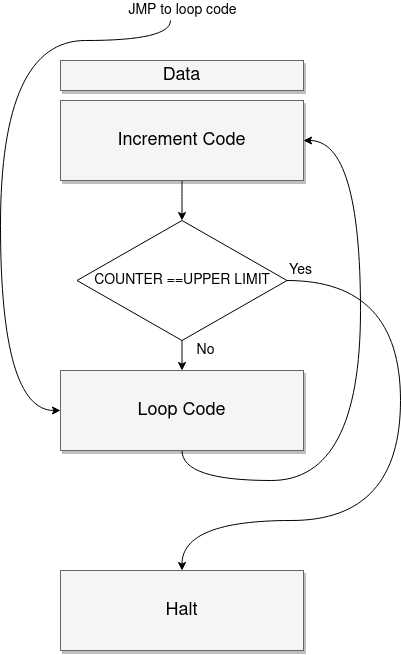
\includegraphics[width=0.4\textwidth]{img/Loop.png}
    \caption{Loop Example Scheme}
    \label{fig:system}
\end{figure}

The following example loops over various instructions to generate the
natural numbers up to a certain value \code{UPPER\_LIMIT} (excluded) and write them on memory starting from a chosen location.
The idea is to fetch from memory a stored value of a \code{COUNTER} (which can be freely initialized), execute "loop" code, increase the counter and perform a comparison with an \code{UPPER\_LIMIT}.
If the counter value is different than the limit, the code enters again the loop. Otherwise, it jumps directly to a halt command, and the program stops.
The loop code fetches an initial address \code{NUMBERS\_ADDR} and uses it to write the current counter value to the address
calculated as \code{NUMBERS\_ADDR + COUNTER}.
In principle, this section could also be substituted by a subroutine call, allowing to implement more complicated operations.

The code is here represented first in pseudo-assembly, and then in explicit Hexadecimal form.
\FloatBarrier
\begin{verbatim}
//jump directly to loop instructions
JMP PTR[LOOP]

//initial counter value, upper limit and memory location to write numbers.
COUNTER = 0 
UPPER_LIMIT = 0A
NUMBERS_ADDR = 35

//code section for counter increment and conditional jump
#INCREMENT# 

//load counter address in H
MVI B,PTR[COUNTER] 
MOV H,B 

//put 01 in B, use it to increase counter by 1, put result in B
MVI B, 01 
ADD B 
MOV B,A 

//write counter to its memory position
MOV M[H],B  

//load upper limit memory location in B, and then the limit itself
MVI B,PTR[UPPER_LIMIT] 
MOV H,B 
MOV B,M[H] 

//compare A (counter) with B(upper limit)
//if A=B, zero flag is set to 1
CMP B 

//check if zero flag is 1 (A=B) and jump to end program if true
CHZ 
JC PTR[AFTER_LOOP]

#LOOP#
//puts counter address in H
MVI B,PTR[COUNTER]
MOV H,B

//puts counter in B, A and C
MOV B, M[H]
MOV A,B
MOV C,B

//load starting address for numbers writing
MVI B,PTR[NUMBERS_ADDR]
MOV H,B
MOV B,M[H]

//calculates address to write counter value, put in H
ADD B
MOV B,A
MOV H,B

//re-load counter value in B and A from C and write it to memory
MOV B,C
MOV A,B
MOV M[H],B

//jump to increment routine
JMP [INCREMENT]

#AFTER_LOOP# 
HLT

#NUMBERS_ADDR#

\end{verbatim}

This is the initial memory state: \\

\noindent\begin{tabular}{ |c| r*{15}{@{ }r}| }
    
        00 & C3 & 15 & 00 & 0A & 35 & 06 & 02 & 60 & 06 & 01 & 80 & 47 & 70 & 06 & 03 & 60 \\ 
        10 & 46 & B8 & CC & DA & 27 & 06 & 02 & 60 & 46 & 78 & 48 & 06 & 04 & 60 & 46 & 80  \\
        20 & 47 & 60 & 41 & 78 & 70 & C3 & 05 & 76 & 00 & 00 & 00 & 00 & 00 & 00 & 00 & 00  \\
        30 & 00 & 00 & 00 & 00 & 00 & 00 & 00 & 00 & 00 & 00 & 00 & 00 & 00 & 00 & 00 & 00\\
        40 & 00 & 00 & 00 & 00 & 00 & 00 & 00 & 00 & 00 & 00 & 00 & 00 & 00 & 00 & 00 & 00\\
    ... \\
        F0 & 00 & 00 & 00 & 00 & 00 & 00 & 00 & 00 & 00 & 00 & 00 & 00 & 00 & 00 & 00 & 00\\
\end{tabular}
\\ \\

While the following is the memory state at the end of the program execution (when the halt \code{HLT} instruction is reached):
\\

\noindent\begin{tabular}{ |c| r*{15}{@{ }r}| }
    
    00 & C3 & 15 & 00 & 0A & 35 & 06 & 02 & 60 & 06 & 01 & 80 & 47 & 70 & 06 & 03 & 60 \\ 
    10 & 46 & B8 & CC & DA & 27 & 06 & 02 & 60 & 46 & 78 & 48 & 06 & 04 & 60 & 46 & 80  \\
    20 & 47 & 60 & 41 & 78 & 70 & C3 & 05 & 76 & 00 & 00 & 00 & 00 & 00 & 00 & 00 & 00  \\
    30 & 00 & 00 & 00 & 00 & 00 & 00 & 01 & 02 & 03 & 04 & 05 & 06 & 07 & 08 & 09 & 00\\
    40 & 00 & 00 & 00 & 00 & 00 & 00 & 00 & 00 & 00 & 00 & 00 & 00 & 00 & 00 & 00 & 00\\
... \\
    F0 & 00 & 00 & 00 & 00 & 00 & 00 & 00 & 00 & 00 & 00 & 00 & 00 & 00 & 00 & 00 & 00\\
\end{tabular}
\\
\\
As it can be seen, after the executon, the values \code{ 0x00, 0x01, .., 0x09 < 0x0A} have been written in memory starting from address \code{0x35}, as expected.
